
%--------------------------------------------------------
%--------------------------------------------------------
%\section{The spin-0 description of CMB polarization} \label{sec:pol-intro}
%--------------------------------------------------------
\section{Polarization primer}\label{sec:pol-primer}
The CMB polarization is measured in terms of Stokes $Q$ and $U$ parameters. Stokes $Q$ is defined as the linear polarization measured along local cartesian axes ($+$ along the $x$-axis and $-$ along the $y$-axis) while Stokes $U$ is defined as the linear polarization measured along the cartesian axes rotated by $45^{\circ}$ ($+$ along x-axis and $-$ along the y-axis in the counter-clockwise rotated system). The Stokes parameters depend on the choice of the coordinate system and two different coordinate systems rotated by an angle $\psi$ relate as
%
\beq \label{eq:qu-rot}
\fqu' = \begin{bmatrix} \cos{2 \psi} &  \sin{2 \psi} \\ -\sin{2\psi} & \cos{2 \psi} \end{bmatrix} \fqu \,.
\eeq
%
%which one can simply checked by verifying that $Q' \rightarrow U$ and $U' \rightarrow -Q$ when the coordinate systems are rotated by $45^\circ$ in the counter-clockwise sense. 

Following the notation of \cite{Zaldarriaga1997}, fields which transform as
%
%\beq
${}_{s}f' = e^{-is\psi} {}_{s}f $
%\eeq
%
under right handed rotations of the local coordinate system are termed spin-$s$ fields. The Stokes parameters can be combined to define the complex fields,
%
\beq \label{eq:spin-pol}
_{\pm 2}\bar{X}(\hat{n}) = Q(\hat{n}) \pm i U (\hat{n}) \,, %\nonumber \\ &=& \sum_{\ell m}  {_{\pm 2}} \tilde{X}_{\ell m}  \, {_{\pm 2}}Y_{\ell m} (\hat{n}) \,.
\eeq
%
which under rotation of the local tangent plane coordinate system by an angle $\psi$ at any point on the sphere transform as: $_{\pm 2}X' = e^{\mp i2\psi} {_{\pm 2}X}$, which follows directly from \eq{eq:qu-rot}. Therefore the quantities $_{\pm2}X$ are spin ${\pm2}$ fields respectively.

The coordinate dependence of Stokes parameters make them inconvenient to work with.  With operations that raise (or lower) the spin of the field, we can produce a spin-0 scalar that is coordinate independent.   The spin-raising operator ($\eth$), when operated on a field of spin-s $_{s}f$, results in a fields with spin-$(s+1)$: $(\eth _{s}f)' = e^{-i(s+1)\psi}(\eth _{s}f)$  \cite{goldberg67}.  The complementary spin-lowering operator $(\bar{\eth})$  similarly results with $(\bar{\eth} _{s}f)' = e^{-i(s-1)\psi}(\bar{\eth} _{s}f)$.  The complex spin-0 scalar now arise from  the spin-2 fields ${_{\pm 2}X}$ as follows,
%
\begin{subequations}\label{eq:ebdef}
\beqry
\mathcal{E}(\hat{n}) + i \mathcal{B}(\hat{n}) &=& -\bar{\eth}^2 _{+ 2}\bar{X}(\hat{n}) \,,\\
\mathcal{E}(\hat{n}) - i \mathcal{B}(\hat{n}) &=& -{\eth}^2 _{-2}\bar{X}(\hat{n}) \,.
\eeqry
\end{subequations}
%
%which by the virtue of being scalars are independent of coordinate definitions. %The real part of this complex spin-0 scalar field corresponds to the E-mode while the imaginary part to the B-modes \cite{Kamionkowski1997}. 

The complex field $_{\pm 2}X$ defined on the sphere can be decomposed in spin spherical harmonic functions: ${}_{\pm 2}X(\hat{n}) = \sum_{\ell m} {}_{\pm 2} X_{\ell m} {}_{\pm 2}Y_{\ell m}(\hat{n})$. On applying the spin raising and lowering operators on the spin spherical harmonic functions leads to the following identities \cite{goldberg67},
%
\begin{subequations}\label{eq:spinopylm} 
\beqry
\eth _s Y_{lm}(\hat{n}) &=& \sqrt{(\ell-s)(\ell+s+1)} _{s+1} Y_{lm}(\hat{n}) \,, \\
\bar{\eth} _s Y_{lm}(\hat{n}) &=& -\sqrt{(\ell+s)(\ell-s+1)} _{s-1} Y_{lm}(\hat{n}) \,, 
\eeqry
\end{subequations}
%
where $_s Y_{lm}(\hat{n}) $ denote the spin-s spherical harmonics.

Using the definition of $\mathcal{E/B}$, the spin spherical harmonic decomposition of ${}_{\pm2}X$ and the identities given in \eq{eq:spinopylm} it can be shown that the scalar fields $\mathcal{E}/\mathcal{B}$ are given by the following equations,
%
\beq \label{eq:pseudo}
\mathcal{E}(\hat{n}) = \sum_{\ell m} a^{E}_{\ell m} \sqrt{\frac{(\ell+2)!}{(\ell-2)!}} Y_{\ell m} (\hat{n}) ~\,;~ \mathcal{B}(\hat{n})  =\sum_{\ell m} a^{B}_{\ell m} \sqrt{\frac{(\ell+2)!}{(\ell-2)!}} Y_{\ell m} (\hat{n}) \,,
\eeq
%
where the harmonic coefficients $a^{E}_{\ell m}$  \& $a^{B}_{\ell m}$ are related to the harmonic coefficients of the spin-2 polarization field via the following equations,
%
\beq\label{eq:x2eb}
a^{E}_{\ell m} = -\frac{1}{2} \Big[ {}_{+2}\tilde{X}_{\ell m} + {}_{-2}\tilde{X}_{\ell m} \Big] ~\,;~a^{B}_{\ell m} = -\frac{1}{2i} \Big[ {}_{+2}\tilde{X}_{\ell m} - {}_{-2}\tilde{X}_{\ell m} \Big] \,.
\eeq
%
In the remainder of this article, we will work with the scalar $E$ and pseudo scalar $B$ fields as defined by the following equations, 
%
\beq \label{eq:realeb}
E(\hat{n}) = \sum_{\ell m} a^{E}_{\ell m} Y_{\ell m} (\hat{n}) ~\,;~ B(\hat{n})  =\sum_{\ell m} a^{B}_{\ell m} Y_{\ell m} (\hat{n}) \,.
\eeq
%
Note that these $E/B$ fields are merely filtered versions of $\mathcal{E}/\mathcal{B}$ as their spherical harmonic coefficients of expansion are related by the factor $[{(\ell+2)!}/{(\ell-2)!}]^{1/2}$. %We make this choice since the CMB spectra are more closely related to the fields E \& B.
%--------------------------------------------------------
%--------------------------------------------------------
%%%%%%%%%%%%%%%%%%%%%%%%%%%%%%%%%%%
\section{Real space operators} \label{sec:real_space_operators}
The vector-matrix notation introduced in  \sec{sec:mat_pol_intro} allows for concise book keeping of all the operations involved in the analysis of CMB polarization. In this section we use this notation to derive the real space operators which translate the Stokes vector \vp{}  to the vector of scalars \vs  and vice versa. This vector-matrix notation also allows us to simply derive real space operators for direct decomposition of the Stokes vector \vp{} in to a vector \vp{ E} that correspond to $E$-modes and another vector \vp{B} that corresponds to the $B$-modes of polarization, such that \vp{} = \vp{E} + \vp{B}, without ever evaluating the $E$ \& $B$ fields or their spherical harmonics. 
All the real space operators we derive are most conveniently expressed as functions of the Euler angles  $\alpha, ~\beta~\&~ \gamma$ on the sphere. Owing to this, we begin with a brief discussion on Euler angles and \revisit{present a visual method to think about them.}
%
\begin{figure}[!hbt]
\centering
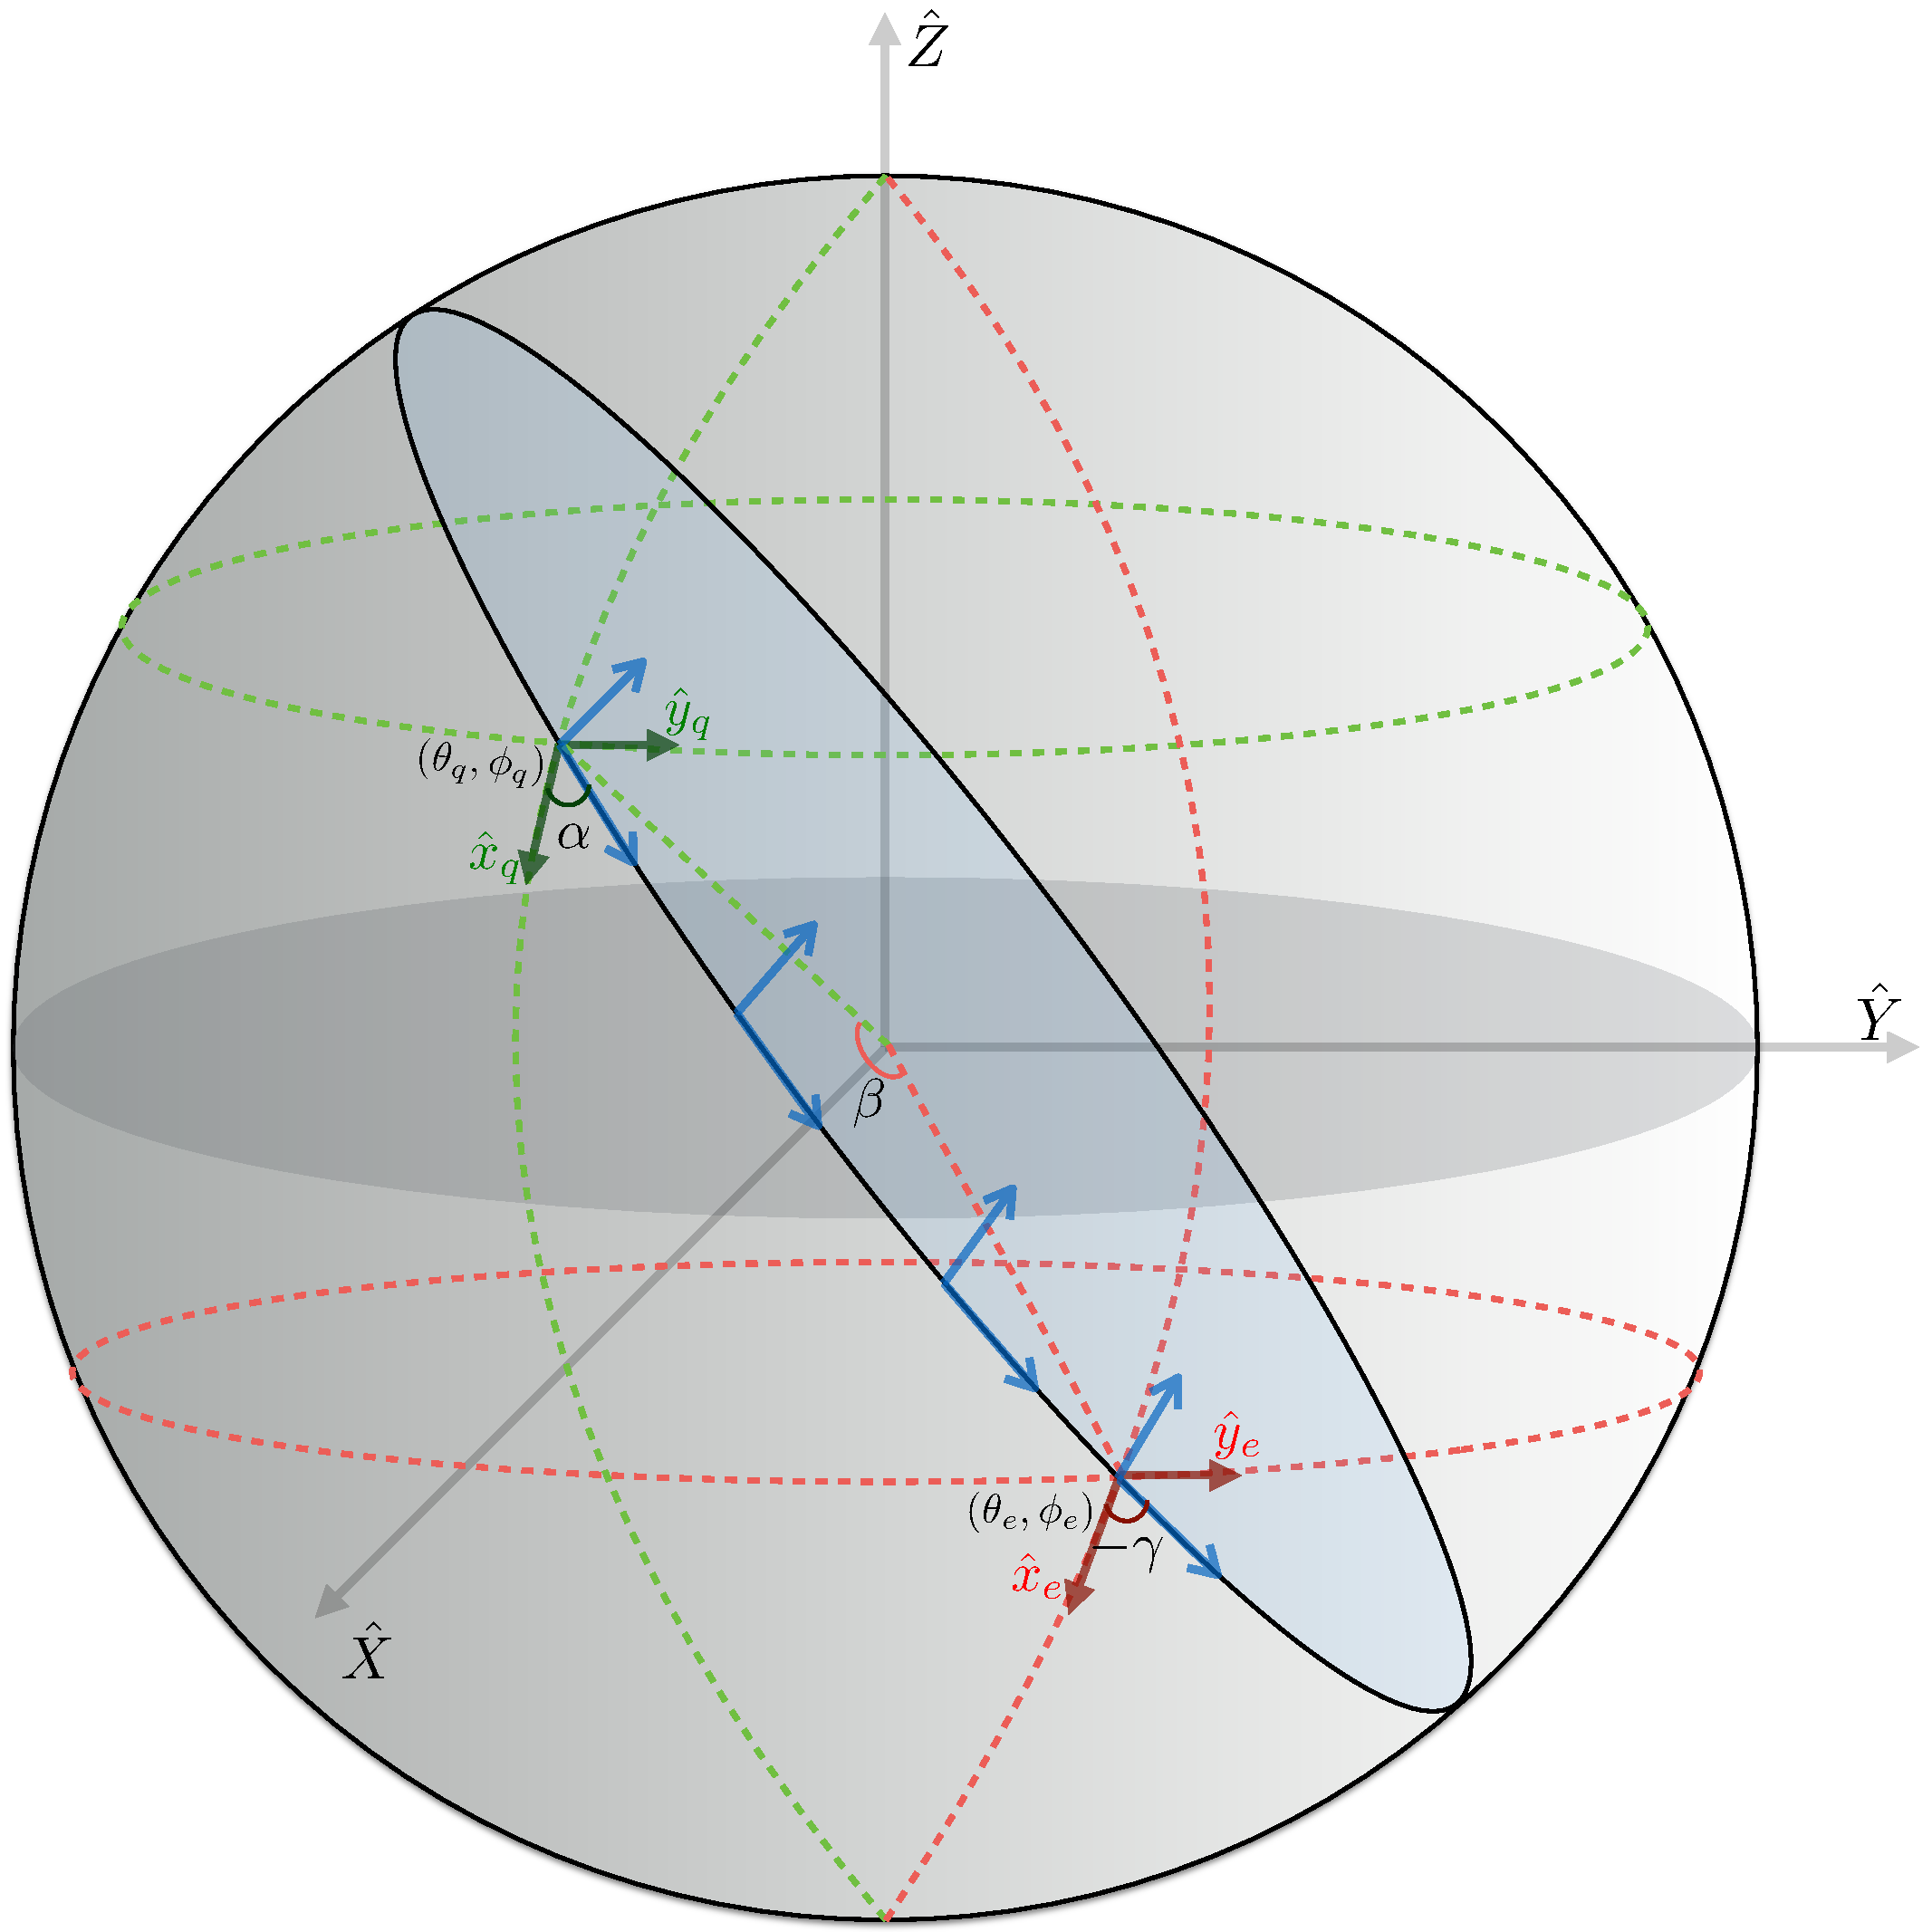
\includegraphics[width=0.5\columnwidth]{euler.pdf}
\caption{This figure depicts the Euler angles in the z-y1-z2 convention. The cartesian coordinates shown in dark green are those that lie in the tangent plane at location $\hat{n}_q = (\theta_q, \phi_q)$ while those shown in dark red are the ones that lie in the tangent plane at location $\hat{n}_e = (\theta_e, \phi_e)$. The blue coordinates at different locations are representative of the parallel transport along the geodesic connection the two locations $\hat{n}_q$ \& $\hat{n}_e$ on the sphere.}
\label{fig:euler_angles}
\end{figure}
%

\textit{Euler angles:}  We define the local cartesian coordinate system at any point on the sphere such that the z-axis points along the radial direction, the x-axis is along the vector tangent to the local longitude pointing south and the y-axis is a vector tangent to the local latitude pointing east as shown in \fig{fig:euler_angles}. The Euler angles $\alpha ,\beta ~\&~ \gamma$ define rotation operations that transforms the local cartesian coordinate system defined at the location $\hat{n}_q \equiv (\theta_q,\phi_q)$ such that it aligns with the local cartesian coordinate system at the location $\hat{n}_e \equiv (\theta_e,\phi_e)$ \cite{varshalovich}. 

For this work, it is convenient to think in the z-y1-z2 convention therefore all future references to Euler angles are in this convention\footnote{The Euler angles in the more standard $z-y-z$ convention are related to those in the $z-y1-z2$ convection by the following rule: $(\alpha,\beta,\gamma)_{z-y-z} =(\gamma,\beta,\alpha)_{z-y1-z2}$ \cite{varshalovich}.}.
In the z-y1-z2 convention, $\alpha$ defines the rotation about the z-axis, $\beta$ defines the rotation about the new y-axis (y1-axis) after the previous rotation and $\gamma$ defines the rotation about the final z-axis (z2-axis) after carrying out the previous two rotations. These angles can be understood as follows: The rotation by $\alpha$ about the original z-axis is such that it aligns the x-axis of the cartesian system at location $\hat{n}_q$ along the great circle in the direction \revisit{of shortest arc length} towards $\hat{n}_e$.  The rotation by $\beta$ about the y2-axis parallel transports the local cartesian coordinate system from location $\hat{n}_q$ to location $\hat{n}_e$, such that the z-axes of the two coordinate systems are parallel to each other. Finally the rotation by angle $\gamma$ about the z2-axis aligns the x \& y axes of the parallel transported system with those of the local cartesian system defined at $\hat{n}_e$. The different Euler angles and the corresponding rotations are schematically represented in \fig{fig:euler_angles}.

The simplest scenario is when one of the coordinates coincides with the north pole $\hat{n}_q=(\theta_q,\phi_q)=(0,0)$ (the local cartesian system at this point being defined with an arbitrary convention set by choosing $\theta_0 \rightarrow 0$ while moving along the longitude $\phi_0=0$), in which case it is easy to see that rotations by Euler angles: $(\alpha,\beta,\gamma) =(\phi_e,\theta_e,0)$ will align the cartesian system at $\hat{n}_q$ with that defined at position $\hat{n}_e$. 
%--------------------------------------------------------

%--------------------------------------------------------
\subsection{A heuristic argument for constructing  $E/B$ modes from Stokes parameters $Q/U$ on the sphere} \label{sec:qu2eb_heuristic}
The primary aim here is to make intuitive the construction of the spin-0 $E/B$ modes of polarization from the Stokes parameters. We present heuristic arguments which allows us to derive the important features of the real space kernels\footnote{These heuristic arguments were developed in hindsight but are very instructive.}. 

If one rotates the cartesian coordinates in the tangent plane at location $\hat{n}_q$ by an angle $\phi$ about the local $\hat{z}_q$ axis, the Stokes charge in the new coordinate system is related to the Stokes charge in the original coordinate system as: ${}_{+2}X'(\hat{n}_q) \xrightarrow{\mathcal{R}_{\hat{z}_q}(\phi)} {}_{+2}X(\hat{n}_q) e^{-i2\phi} $. Similarly if the local planar axes are rotated by an angle $\phi$ then the Euler angle $\alpha_{qe}$ (recall that this Euler angle aligns the x-axis at $\hat{n}_q$ in the direction of the shortest path along the geodesic to the location $\hat{n}_e$) for the new coordinate system is given by: $\alpha'_{qe} \rightarrow \alpha_{qe} - \phi$ and therefore one can see that: $e^{-i2\alpha'_{qe}} \xrightarrow{\mathcal{R}_{\hat{z}_q}(\phi)} e^{-i2\alpha_{qe}} e^{i2\phi}$. The Euler angles $|\beta_{qe}|$ which measure the angular distance between pixels remains unaltered under this local rotation operation.  Given these transformation properties note that: ${}_{+2}X'(\hat{n}_q)e^{-i2\alpha'_{qe}} \xrightarrow{\mathcal{R}_{\hat{z}_q}(\phi)} {}_{+2}X(\hat{n}_q) e^{-i2\alpha_{qe}}$ is invariant under rotations  $\mathcal{R}_{\hat{z}_q}(\phi)$ and hence by definition must form a spin-0 field.  Now note that the real part of the function are constructed by product of functions $(Q\cos{2\alpha}, U\sin{2 \alpha})$ having the same parity and hence the real part must have even parity while the imaginary part of the function are constructed by multiplying functions $(Q\sin{2 \alpha}, U\cos{2\alpha})$ of opposite parity and hence must have an odd parity. Therefore we can make the association: $E'+iB' \propto {}_{+2}X(\hat{n}_q) e^{-i2\alpha_{qe}}$

Now note that when the two locations coincide $\hat{n}_q = \hat{n}_e$ then  $\alpha_{qe}=0,2\pi,4\pi,\cdots$ implying $E + iB \propto Q+iU$, which is a fallacy as we know that $Q+iU$ does not transform as a spin-0 field under local rotations. One runs into a similar fallacy when the two locations are diametrically opposite.  Therefore to have a consistent definition of a spin-0 field constructed from a spin-2 field we require the kernel to have the form: $E'+iB' = {}_{+2}X(\hat{n}_q) f(\beta_{qe})  e^{-i2\alpha_{qe}}$, where the function $f(\beta_{qe})$ is such that it vanishes when the two locations are coincident$(\beta_{qe}=0)$ or diametrically opposite$(\beta_{qe}=\pi)$. Hence the $E/B$ fields are necessarily non-local. Note that this construction can be generalized to transform fields of arbitrary spin to a field of any other spin, one obvious case being constructing the Stokes field given the $E/B$ maps (i.e. deriving spin-2 fields from spin-0 fields.)

The azimuthal part which depends only on the Euler angle $\alpha_{qe}$, has no multipole $\ell$ dependence and is the crucial operation which translates between the different spin representation of CMB polarization. Only the radial part of the kernel $f(\beta_{qe})$ depends only on the angular separation $|\beta_{qe}|$ between different locations on the sphere and hence must completely incorporate the multipole $\ell$ dependence of the kernel. These heuristic arguments cannot take us any further and we now shift to presenting a mathematically rigorous derivation of the real space operators in the following sections. 
%--------------------------------------------------------
